%%%%%%%%%%%%%%%%%%%%%%%%%%%%%%%%%%%%%%%%%
% Beamer Presentation
% LaTeX Template
% Version 1.0 (10/11/12)
%
% This template has been downloaded from:
% http://www.LaTeXTemplates.com
%
% License:
% CC BY-NC-SA 3.0 (http://creativecommons.org/licenses/by-nc-sa/3.0/)
%
%%%%%%%%%%%%%%%%%%%%%%%%%%%%%%%%%%%%%%%%%

%----------------------------------------------------------------------------------------
%	PACKAGES AND THEMES
%----------------------------------------------------------------------------------------

\documentclass{beamer}

\usepackage[brazilian]{babel}
\usepackage[utf8]{inputenc}
\usepackage[T1]{fontenc}
\usepackage{colortbl}

\mode<presentation> {

% The Beamer class comes with a number of default slide themes
% which change the colors and layouts of slides. Below this is a list
% of all the themes, uncomment each in turn to see what they look like.

%\usetheme{default}
%\usetheme{AnnArbor}
%\usetheme{Antibes}
%\usetheme{Bergen}
%\usetheme{Berkeley}
%\usetheme{Berlin}
%\usetheme{Boadilla}
%\usetheme{CambridgeUS}
%\usetheme{Copenhagen}
%\usetheme{Darmstadt}
%\usetheme{Dresden}
\usetheme{Frankfurt}
%\usetheme{Goettingen}
%\usetheme{Hannover}
%\usetheme{Ilmenau}
%\usetheme{JuanLesPins}
%\usetheme{Luebeck}
%\usetheme{Madrid}
%\usetheme{Malmoe}
%\usetheme{Marburg}
%\usetheme{Montpellier}
%\usetheme{PaloAlto}
%\usetheme{Pittsburgh}
%\usetheme{Rochester}
%\usetheme{Singapore}
%\usetheme{Szeged}
%\usetheme{Warsaw}

% As well as themes, the Beamer class has a number of color themes
% for any slide theme. Uncomment each of these in turn to see how it
% changes the colors of your current slide theme.

%\usecolortheme{albatross}
%\usecolortheme{beaver}
%\usecolortheme{beetle}
%\usecolortheme{crane}
%\usecolortheme{dolphin}
%\usecolortheme{dove}
%\usecolortheme{fly}
%\usecolortheme{lily}
%\usecolortheme{orchid}
%\usecolortheme{rose}
%\usecolortheme{seagull}
%\usecolortheme{seahorse}
%\usecolortheme{whale}
%\usecolortheme{wolverine}

%\setbeamertemplate{footline} % To remove the footer line in all slides uncomment this line
%\setbeamertemplate{footline}[page number] % To replace the footer line in all slides with a simple slide count uncomment this line

%\setbeamertemplate{navigation symbols}{} % To remove the navigation symbols from the bottom of all slides uncomment this line
}

\usepackage{graphicx} % Allows including images
\usepackage{booktabs} % Allows the use of \toprule, \midrule and \bottomrule in tables

%----------------------------------------------------------------------------------------
%	TITLE PAGE
%----------------------------------------------------------------------------------------

\title[Apresentação do Curso]{Métodos de Otimização (ENE081) - Turma B} 

\author{Prof. André Luís Marques Marcato} % Your name
\institute[UFJF/PPEE]{Universidade Federal de Juiz de Fora \\
					  Programa de Pós-Graduação em Engenharia Elétrica \\
\medskip
\textit{\href{mailto:andre.marcato@ufjf.edu.br}{andre.marcato@ufjf.edu.br}}
}
\date{\today}

\begin{document}
\begin{frame}
\titlepage % Print the title page as the first slide
\begin{figure}[!htb]
\centering
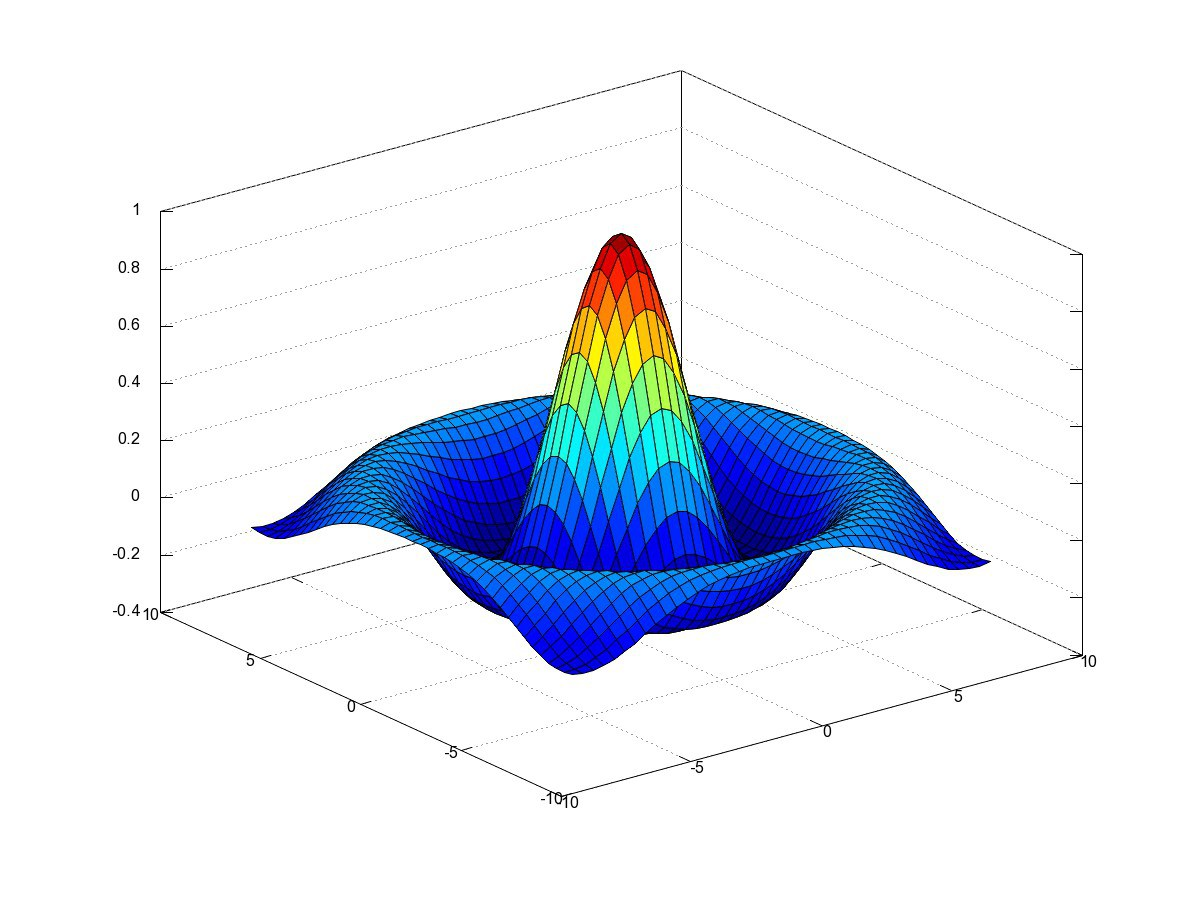
\includegraphics[width=5cm, height=3cm]{cover.jpg}
\end{figure}
\end{frame}

\begin{frame}
\frametitle{Agenda da Apresentação} % Table of contents slide, comment this block out to remove it
\tableofcontents % Throughout your presentation, if you choose to use \section{} and \subsection{} commands, these will automatically be printed on this slide as an overview of your presentation
\end{frame}

%----------------------------------------------------------------------------------------
%	PRESENTATION SLIDES
%----------------------------------------------------------------------------------------

%------------------------------------------------
\section{Objetivos} 

\subsection{O que vamos estudar?} 

\begin{frame}
\frametitle{Principais Tópicos}
\begin{itemize}
\item Programação Linear\\~\\

\item Programação Inteira\\~\\

\item Programação Não Linear\\~\\

\item Programação Dinâmica\\~\\

\item Otimização Baseada em Inteligência Computacional\\~\\

\item Transversalmente: Utilizar Matlab ou Python

\end{itemize}
\end{frame}

%------------------------------------------------

\section{Referências Bibliográficas}
\subsection{Relação de livros sobre o tema} 

\begin{frame}
\frametitle{Referência Principal}

\begin{figure}[!htb]
\centering
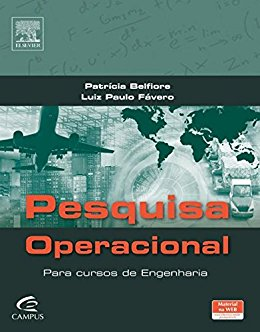
\includegraphics[width=4cm, height=6cm]{pesquisaoperacional-campus.jpg}
\caption{Patrícia Belfiore e Luiz Paulo Fávero, Pesquisa Operacional para Cursos de Engenharia, Elsevier, 2013.}
\end{figure}

\end{frame}

\begin{frame}
\frametitle{Referências Secundárias}
\centering

\only<1>
{
	\begin{figure}[!htb]
		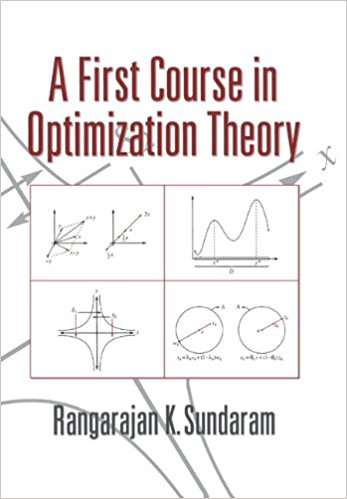
\includegraphics[width=4cm, height=6cm]{a-first-course-in-optimization-theory.jpg}
	\end{figure}
}

\only<2>
{
	\begin{figure}[!htb]
		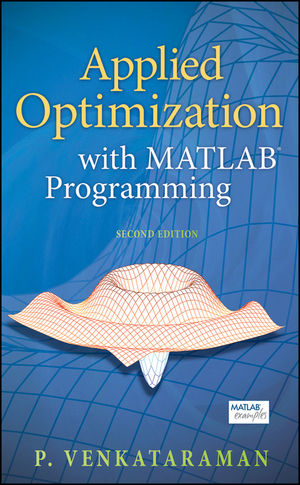
\includegraphics[width=4cm, height=6cm]{Applied-Optimization-with-MATLAB-Programming-SDL069600218-1-c62c2.jpg}
	\end{figure}
}

\only<3>
{
	\begin{figure}[!htb]
		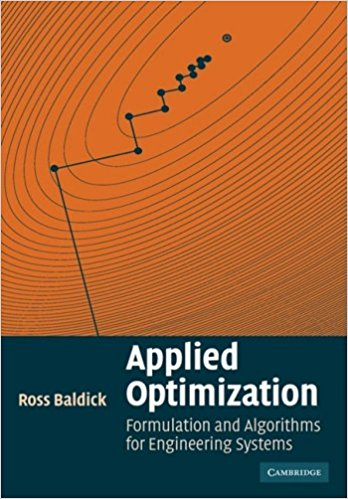
\includegraphics[width=4cm, height=6cm]{appliedoptmization.jpg}
	\end{figure}
}

\only<4>
{
	\begin{figure}[!htb]
		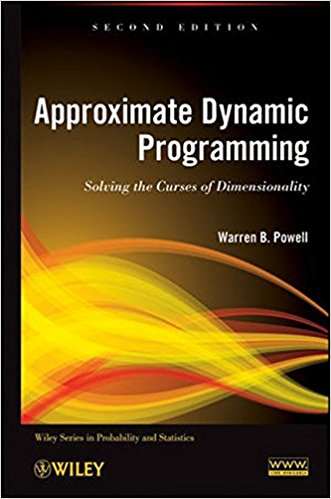
\includegraphics[width=4cm, height=6cm]{aproximatesdp.jpg}
	\end{figure}
}
\only<5>
{
	\begin{figure}[!htb]
		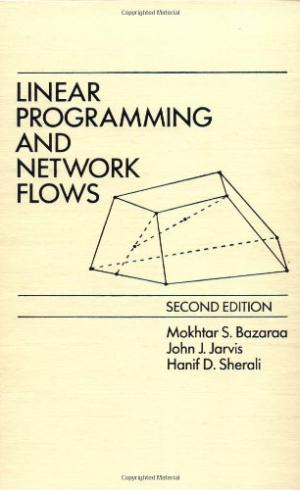
\includegraphics[width=4cm, height=6cm]{bazaraa.jpg}
	\end{figure}
}

\only<6>
{
	\begin{figure}[!htb]
		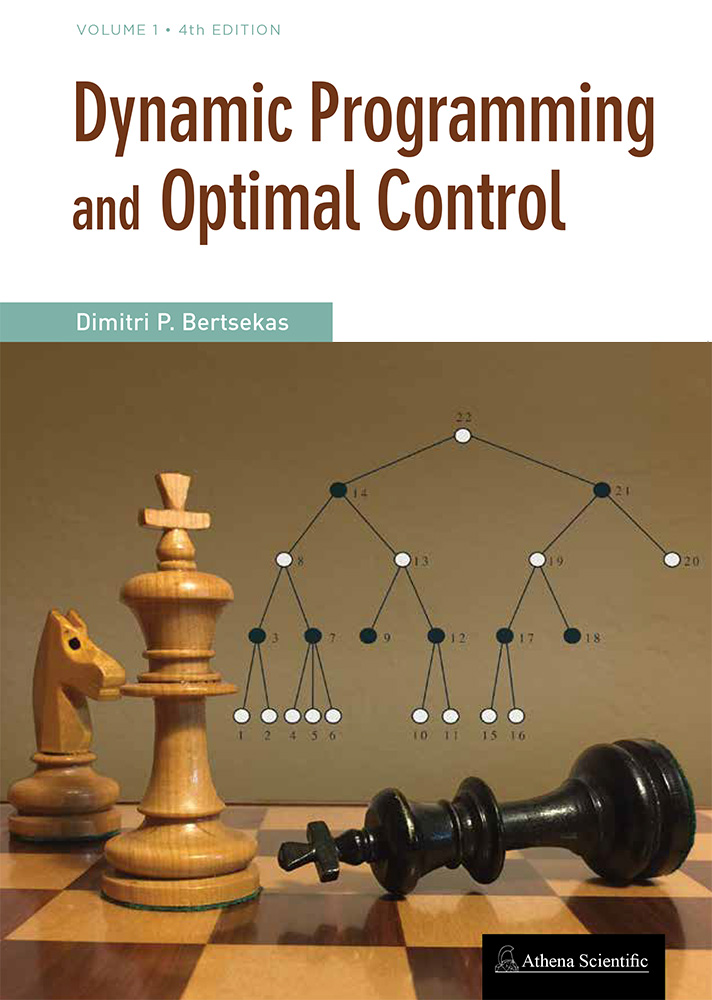
\includegraphics[width=4cm, height=6cm]{bertsekas_0.jpg}
	\end{figure}
}
\only<7>
{
	\begin{figure}[!htb]
		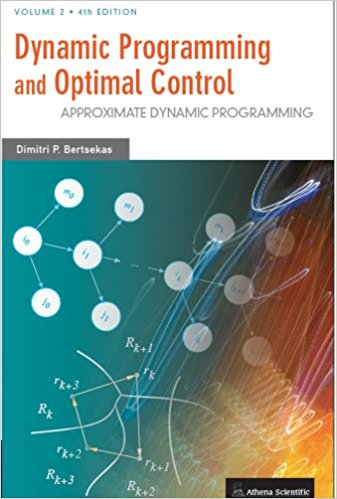
\includegraphics[width=4cm, height=6cm]{bertsekas_1.jpg}
	\end{figure}
}

\only<8>
{
	\begin{figure}[!htb]
		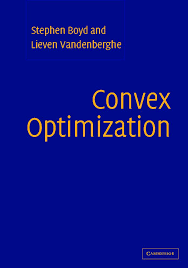
\includegraphics[width=4cm, height=6cm]{convexoptmization.png}
	\end{figure}
}

\only<9>
{
	\begin{figure}[!htb]
		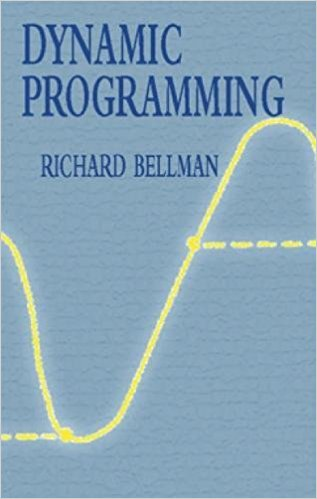
\includegraphics[width=4cm, height=6cm]{dynamicprogramming-belmann.jpg}
	\end{figure}
}

\only<10>
{
	\begin{figure}[!htb]
		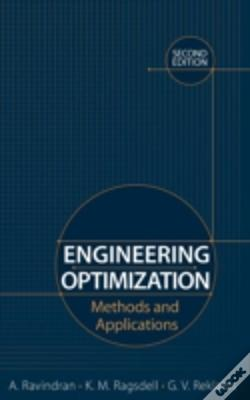
\includegraphics[width=4cm, height=6cm]{engineeringoptimization.jpg}
	\end{figure}
}
\only<11>
{
	\begin{figure}[!htb]
		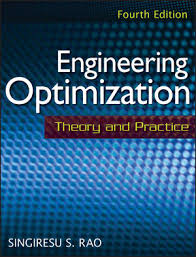
\includegraphics[width=4cm, height=6cm]{engineeringoptmizationrao.jpg}
	\end{figure}
}

\only<12>
{
	\begin{figure}[!htb]
		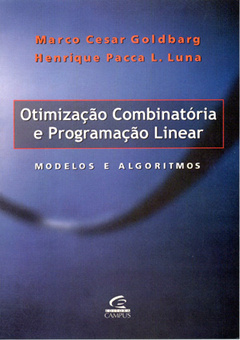
\includegraphics[width=4cm, height=6cm]{goldberg.jpg}
	\end{figure}
}

\only<13>
{
	\begin{figure}[!htb]
		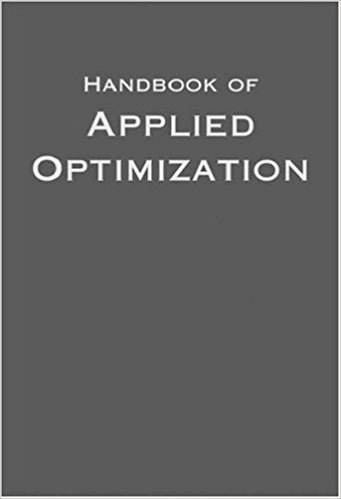
\includegraphics[width=4cm, height=6cm]{handbookofappliedoptmization.jpg}
	\end{figure}
}

\only<14>
{
	\begin{figure}[!htb]
		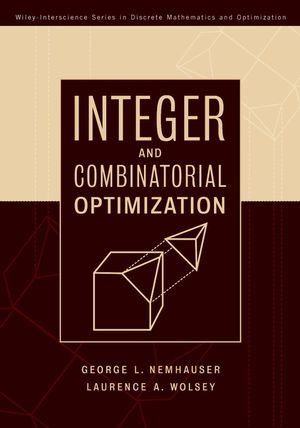
\includegraphics[width=4cm, height=6cm]{integerandcombinatorial.jpg}
	\end{figure}
}


\only<15>
{
	\begin{figure}[!htb]
		
\includegraphics[width=4cm, height=6cm]{introductiontosdp.jpg}
	\end{figure}
}

\only<16>
{
	\begin{figure}[!htb]
		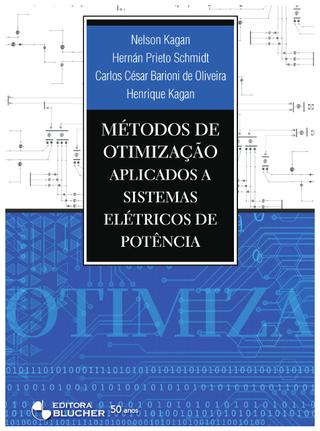
\includegraphics[width=4cm, height=6cm]{kagan.jpg}
	\end{figure}
}

\only<17>
{
	\begin{figure}[!htb]
		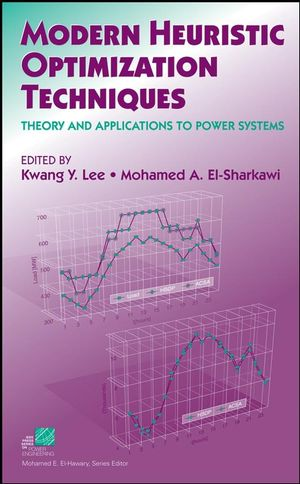
\includegraphics[width=4cm, height=6cm]{modernheuristiques.jpg}
	\end{figure}
}

\only<18>
{
	\begin{figure}[!htb]
		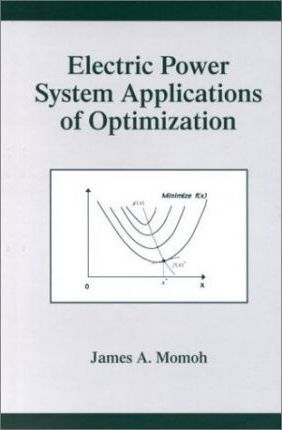
\includegraphics[width=4cm, height=6cm]{momoh.jpg}
	\end{figure}
}

\only<19>
{
	\begin{figure}[!htb]
		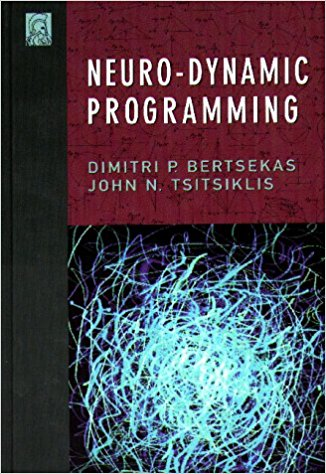
\includegraphics[width=4cm, height=6cm]{neurobertsekas.jpg}
	\end{figure}
}

\only<20>
{
	\begin{figure}[!htb]
		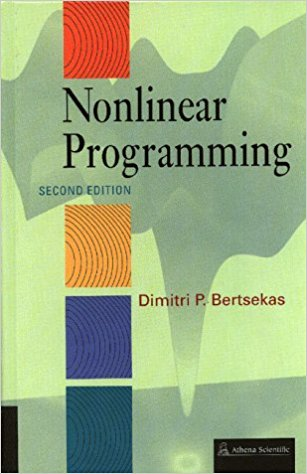
\includegraphics[width=4cm, height=6cm]{nonlinearprogramming.jpg}
	\end{figure}
}

\only<21>
{
	\begin{figure}[!htb]
		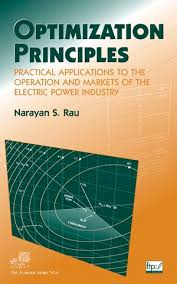
\includegraphics[width=4cm, height=6cm]{optimizationprinciples.jpg}
	\end{figure}
}

\only<22>
{
	\begin{figure}[!htb]
		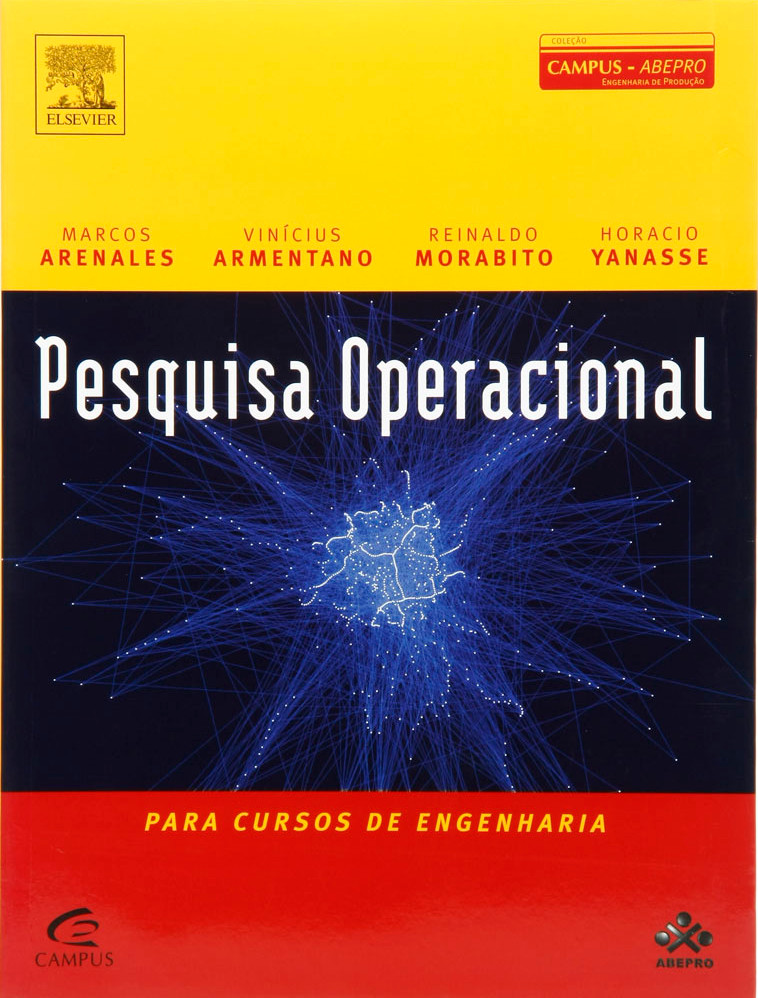
\includegraphics[width=4cm, height=6cm]{Pesquisa-Operacional-Para-Cursos-de-Engenharia-118182.jpg}
	\end{figure}
}

\only<23>
{
	\begin{figure}[!htb]
		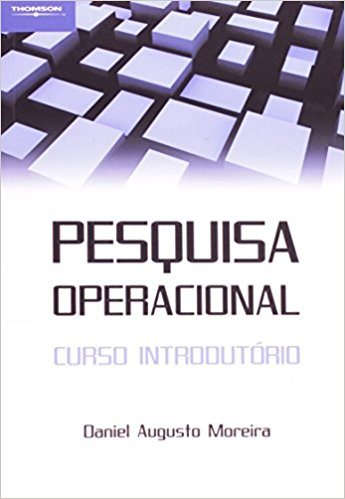
\includegraphics[width=4cm, height=6cm]{pesquisaoperacionalmoreira.jpg}
	\end{figure}
}

\only<24>
{
	\begin{figure}[!htb]
		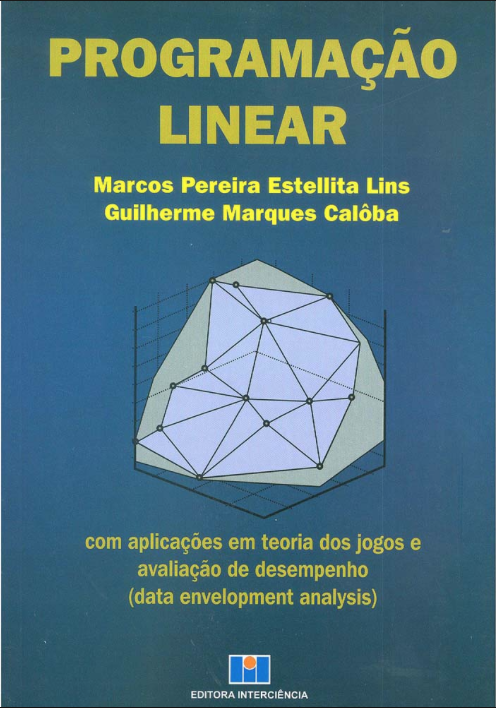
\includegraphics[width=4cm, height=6cm]{programacaolinearcaloba.png}
	\end{figure}
}

\only<25>
{
	\begin{figure}[!htb]
		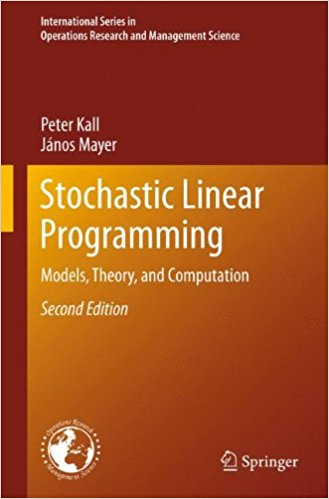
\includegraphics[width=4cm, height=6cm]{sthocasticlinearprogramming.jpg}
	\end{figure}
}

\only<26>
{
	\begin{figure}[!htb]
		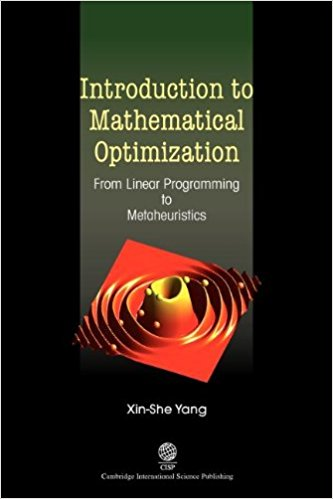
\includegraphics[width=4cm, height=6cm]{introductiontomathematicaloptmization.jpg}
	\end{figure}
}

\only<27>
{
	\begin{figure}[!htb]
		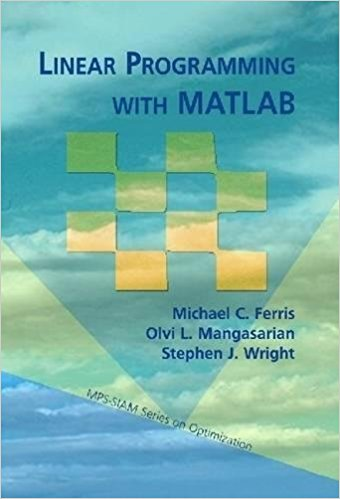
\includegraphics[width=4cm, height=6cm]{linearprogrammingwithmatlab.jpg}
	\end{figure}
}

\only<28>
{
	\begin{figure}[!htb]
		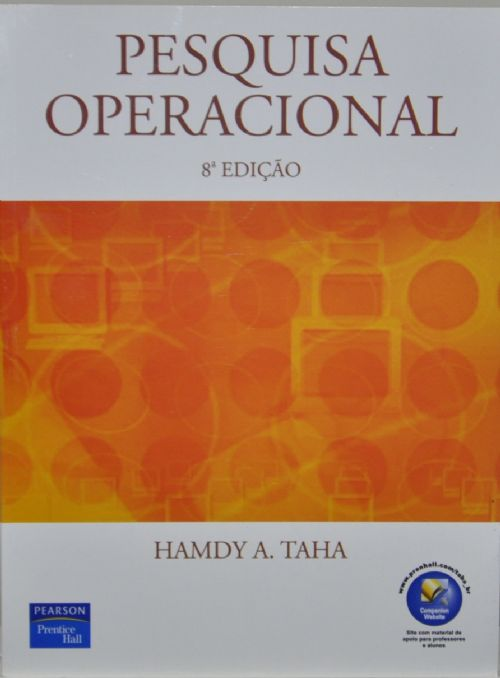
\includegraphics[width=4cm, height=6cm]{pesquisaoperacionalpearson.jpg}
	\end{figure}
}

\only<29>
{
	\begin{figure}[!htb]
		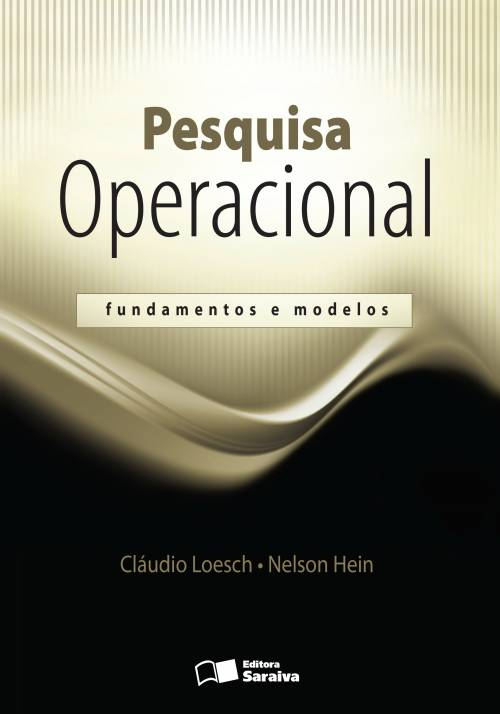
\includegraphics[width=4cm, height=6cm]{pesquisaoperacionalsaraiva.jpg}
	\end{figure}
}

\only<30>
{
	\begin{figure}[!htb]
		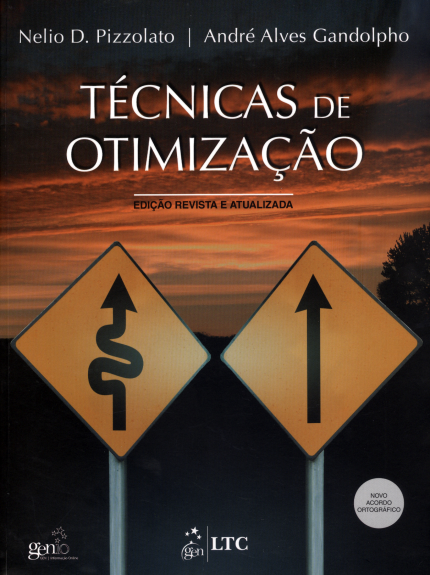
\includegraphics[width=4cm, height=6cm]{tecnicasdeotimizacao.png}
	\end{figure}
}


\end{frame}
%------------------------------------------------

\section{Ementa}
\subsection{ENE081 - Métodos de Otimização - Departamento de Energia - Faculdade de Engenharia - UFJF}

\begin{frame}
	\frametitle{Ementa}
	\begin{block}{Programação Linear}
		\begin{itemize}
			\item Histórico
			\item Modelo Geral de Problemas de Programação Linear
			\item Técnicas de Modelagem
			\item Fundamentos Matemáticos
		\end{itemize}
	\end{block}
\end{frame}

\begin{frame}
	\frametitle{Ementa}
	\begin{block}{Método Simplex}
		\begin{itemize}
			\item Teoria formal do método simplex
			\item O Algoritmo Simplex
			\item Tableau Simplex
			\item O Simplex Compacto
			\item Análise de Sensibilidade/Dualidade na Programação Linear
		\end{itemize}
	\end{block}
\end{frame}

\begin{frame}
	\frametitle{Ementa}
	\begin{block}{Programação Inteira}
		\begin{itemize}
			\item A técnica da ramificação e limite (Branch-and-Bound)
			\item Limites de pesquisa para a ramificação
			\item Algoritmo da ramificação e limite
		\end{itemize}
	\end{block}
\end{frame}

\begin{frame}
	\frametitle{Ementa}
	\begin{block}{Programação Não Linear}
		\begin{itemize}
			\item Modelo de Programação Não Linear
			\item As Condições de Kuhu-Tucker
			\item Método do Gradiente Descendente
			\item Otimização com Restrições (penalidade e barreira)
			\item Método de Pontos Interiores
		\end{itemize}
	\end{block}
\end{frame}

\begin{frame}
	\frametitle{Ementa}
	\begin{block}{Programação Dinâmica}
		\begin{itemize}
			\item Definições
			\item Princípio de Otimalidade
			\item Programação Dinâmica Determinística
			\item Programação Dinâmica Probabilística
		\end{itemize}
	\end{block}
	\begin{block}{Métodos Modernos de Otimização}
		\begin{itemize}
			\item Algoritmos Genéticos
		\end{itemize}
	\end{block}
\end{frame}

\begin{frame}
	\frametitle{Ciência da Gestão Organizacional}
	\begin{itemize}
		\item O processo de tomar decisões gerenciais em bases racionais pressupõe a existência de uma ciência própria, a \textbf{\color{red}Ciência da Gestão}
		\item É comum atribuir-se a Frederick Taylor, um obstinado pela eficiência, pelo combate ao desperdício e pelo melhor uso dos recursos produtivos, que em 1911 publicou o livro Princípios da Administração Científica, o marco inicial da ciência da gestão
	\end{itemize}
	\begin{figure}
		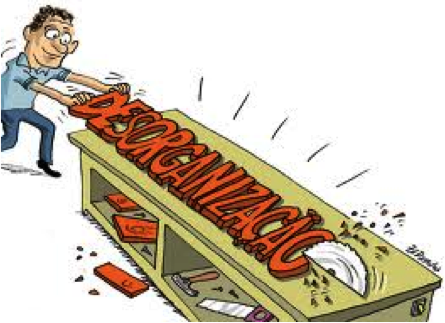
\includegraphics[width=4cm,height=2.5cm]{desorganizacao.png}
	\end{figure}
\end{frame}

\begin{frame}
	\frametitle{Pesquisa Operacional}
	\begin{block}{Segundo www.dictionarybarn.com}
	“Grupo de técnicas desenvolvidas para aplicar ferramentas e métodos científicos para resolver problemas de tomada de decisão em organizações e sistemas complexos. A Pesquisa Operacional busca soluções ótimas em situações de objetivos conflitantes e faz uso de modelos matemáticos a partir dos quais se podem derivar soluções para problemas reais.”
	\end{block}
\end{frame}

\begin{frame}
	\frametitle{Pesquisa Operacional}
	\begin{itemize}
	\item Certamente, o ato de refletir, avaliar consequências e decidir é um distintivo do ser humano 
	\item Mas a criação de metodologias específicas para promover o gerenciamento de decisões é um processo recente, que data da Segunda Guerra Mundial, atendendo pelo nome de \textbf{\color{red}Pesquisa Operacional}, abreviado por \textbf{\color{red}PO}.
	\end{itemize}
\end{frame}

\begin{frame}
	\frametitle{Pesquisa Operacional}
	\begin{itemize}
	\item O marco definitivo na afirmação da Pesquisa Operacional foi a publicação, por George Dantzig, em 1947, do Método Simplex para a \textbf{\color{red}Programação Linear}.
	\end{itemize}
	\begin{figure}
		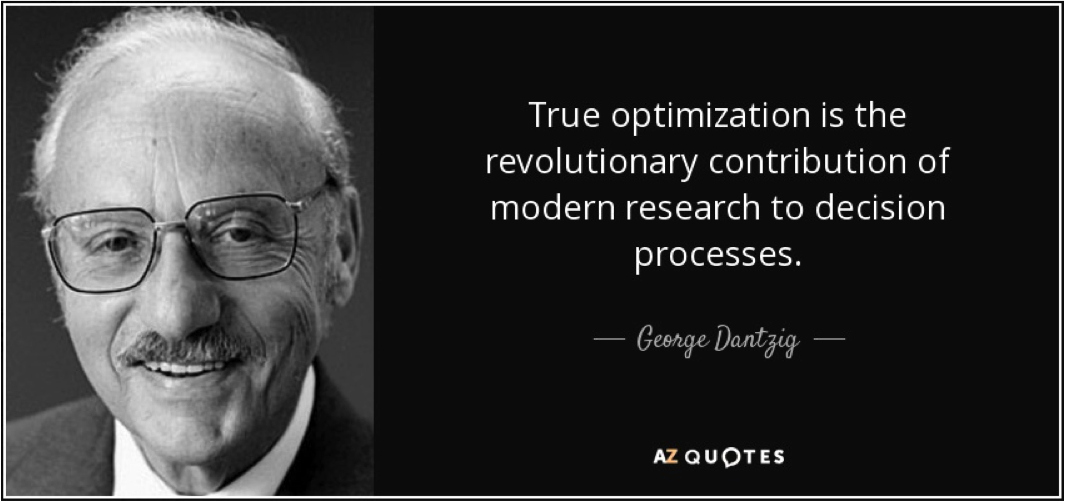
\includegraphics[width=10cm, height=6cm]{dantzig.png}
	\end{figure}
\end{frame}

\begin{frame}
	\frametitle{Os Modelos em PO}
	\begin{itemize}
	\item Em estudos de PO, o uso de modelos faz parte da própria essência.
	\item Trata-se de um recurso adotado para problemas complexos que desafiam a criatividade humana.
	\end{itemize}
	\begin{figure}
		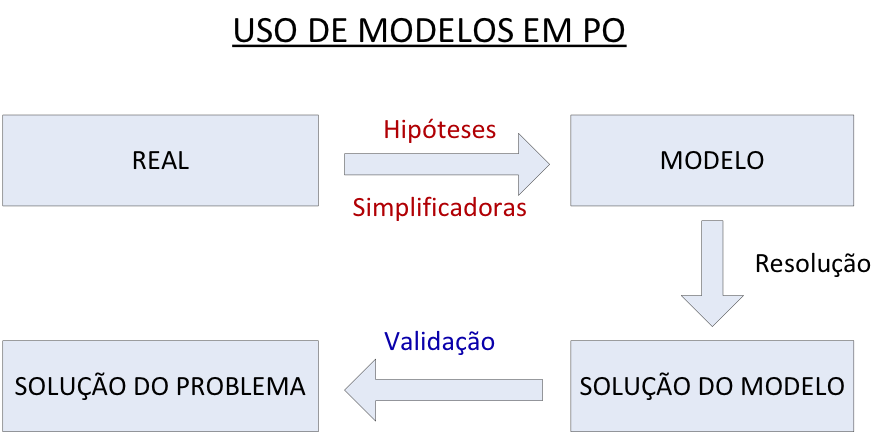
\includegraphics[width=7cm, height=4cm]{modelosPO.png}
	\end{figure}	
	\begin{itemize}
	\item Pode-se dizer que, ao se construir um modelo, passa-se do mundo real ao virtual, \textbf{\color{red}mediante simplificações} que viabilizam essa elaboração conceitual e sua avaliação subsequente.
	\end{itemize}
\end{frame}

\begin{frame}	
	\frametitle{Problemas de Otimização}
	\begin{itemize}
	\item Otimização pode ser definida como a ciência de determinar as \textbf{\color{red}“melhores” soluções} para certos problemas que são formulados matematicamente, em geral, modelos matemáticos de \textbf{\color{red}realizações físicas}.
	\end{itemize}
\end{frame}

\begin{frame}
	\frametitle{Problemas de Otimização}
	\begin{itemize}
	\item {O assunto otimização envolve}
		\begin{itemize}
		\item[*] O estudo de \textbf{\color{red}critérios de otimalidade} para os mais diversos tipos de problemas
		\item[*] A determinação de métodos de solução
		\item[*] O estudo da estrutura destes métodos
		\item[*] \textbf{\color{red}Experimentações computacionais com os métodos de solução aplicados tanto a problemas testes quanto a problemas do mundo real}
		\end{itemize}
	\end{itemize}
\end{frame}

\begin{frame}
	\frametitle{Problemas de Otimização}
	\begin{itemize}
	\item {Áreas de Aplicação}
		\begin{itemize}
		\item[*] Área Militar
		\item[*] Indústria Petrolífera
		\item[*] Indústria de Alimentos
		\item[*] Indústria Siderúrgica
		\item[*] Telecomunicações
		\item[*] Energia Elétrica
		\item[*] Transportes
		\item[*] Robótica
		\item[*] Entre muitos e muitos outros
		\end{itemize}
	\end{itemize}
\end{frame}

%------------------------------------------------

\section{Avaliação}
\subsection{Provas, trabalhos e listas}

\begin{frame}
\frametitle{Regime de Avaliação}
\begin{columns}[c] % The "c" option specifies centered vertical alignment while the "t" option is used for top vertical alignment

\column{.45\textwidth} % Left column and width
\textbf{Provas}
\begin{enumerate}
\item $TVC_1$ (Valor 100 ptos)
\item $TVC_2$ (Valor 100 ptos)
\item $TVC_3$ (Valor 100 ptos)
\end{enumerate} 

\begin{block}{Cálculo da Nota Final}
$Nota = \frac{TVC_1+TVC_2+TVC_3}{3}$ \\~\\

** Em cada TVC, de 10 a 20 pontos serão referentes a trabalhos e/ou listas

\end{block}


\column{.5\textwidth} % Right column and width
\begin{block}{Observações}
\begin{itemize}

\item Com justificativas apresentadas em prazo regulamentar e previstas no RAG, o aluno poderá solicitar segunda chamada com conteúdo apenas da prova perdida.
\item O aluno ausentando-se de um TVC fará prova de segunda chamada no final do período com a matéria toda.
\end{itemize}
\end{block}

\end{columns}

\end{frame}

\begin{frame}
	\textbf{Datas das Provas}
	\begin{enumerate}
		\item $TVC_1$: 10/04/2018 - Quinta - (Anfiteatro Grande - Cantina)
		\item $TVC_2$: 24/05/2018 - Quinta - (Anfiteatro Grande - Cantina)
		\item $TVC_3$: 03/07/2018 - Quinta - (Anfiteatro Grande - Cantina)
		\item $2^a$ Chamada: 05/07/2018 - Quinta - (Anf. Grande - Cantina)
	\end{enumerate}
\end{frame}


\begin{frame}
	\frametitle{Sobre a Segunda Chamada}
	\begin{figure}
		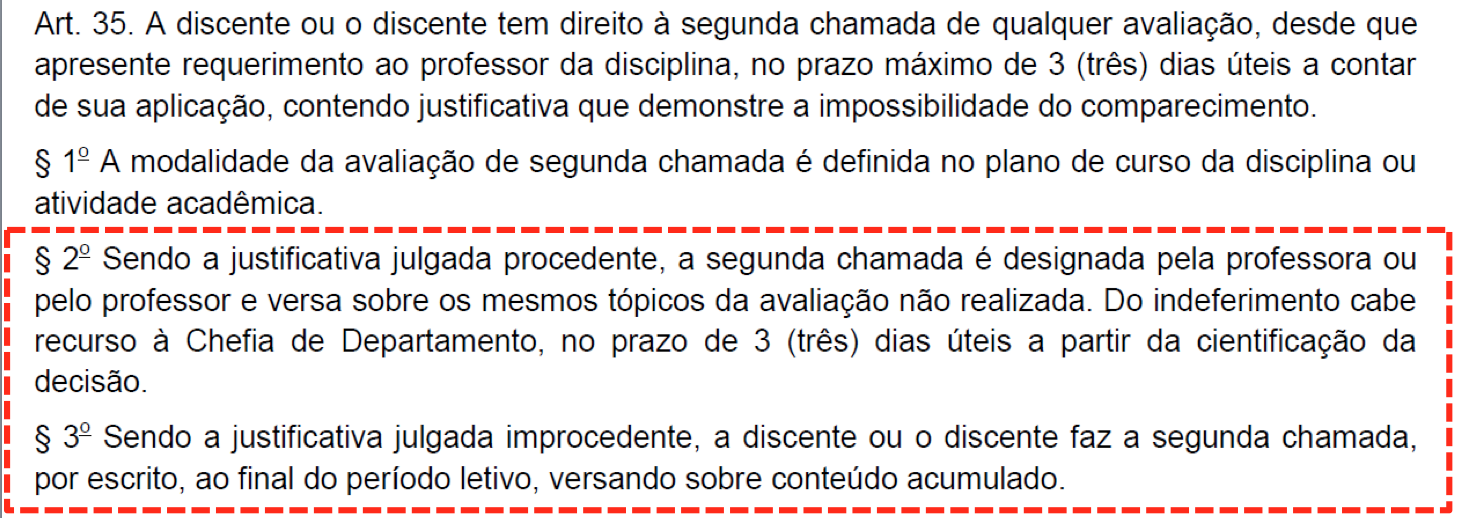
\includegraphics[width=11.5cm, height=6cm]{SegChamada.png}
	\end{figure}
\end{frame}

%------------------------------------------------
\section{Programação do Curso}
\subsection{Dias de Aula}
%------------------------------------------------

\begin{frame}
\frametitle{Calendário 2018/1}
\begin{table}
\begin{tabular}{c c c c c}
\toprule
\textbf{Março} & \textbf{Abril} & \textbf{Maio} & \textbf{Junho} & \textbf{Julho}\\
\midrule
\cellcolor{green}06 & \cellcolor{green}03   & \cellcolor{cyan}01    & \cellcolor{green}05 & \cellcolor{magenta}03 \\
\cellcolor{green}08 & \cellcolor{green}05   & \cellcolor{green}03   & \cellcolor{green}07 & \cellcolor{magenta}05 \\
\cellcolor{green}13 & \cellcolor{magenta}10 & \cellcolor{green}08   & \cellcolor{green}12 & \cellcolor{yellow}07 \\
\cellcolor{green}15 & \cellcolor{green}12   & \cellcolor{green}10   & \cellcolor{green}14 & \cellcolor{gray}-- \\
\cellcolor{green}20 & \cellcolor{green}17   & \cellcolor{green}15   & \cellcolor{green}19 & \cellcolor{gray}-- \\
\cellcolor{green}22 & \cellcolor{green}19   & \cellcolor{green}17   & \cellcolor{green}21 & \cellcolor{gray}-- \\
\cellcolor{green}27 & \cellcolor{green}24   & \cellcolor{yellow}22  & \cellcolor{green}26 & \cellcolor{gray}-- \\
\cellcolor{cyan}29  & \cellcolor{green}26   & \cellcolor{magenta}24 & \cellcolor{green}28 & \cellcolor{gray}-- \\
\cellcolor{white}-- & \cellcolor{white}--   & \cellcolor{green}29   & \cellcolor{white}-- & \cellcolor{gray}-- \\
\cellcolor{white}-- & \cellcolor{white}--   & \cellcolor{cyan}31    & \cellcolor{white}-- & \cellcolor{gray}-- \\
\bottomrule
\cellcolor{green}Aula & \cellcolor{magenta}Prova & \cellcolor{cyan}Recesso & \cellcolor{yellow}Não Houve & \cellcolor{gray}Férias\\
\end{tabular}
\end{table}
\end{frame}

%------------------------------------------------

\begin{frame}
\Huge{\centerline{Fim}}
\end{frame}

%----------------------------------------------------------------------------------------

\end{document} 